
%(BEGIN_QUESTION)
% Copyright 2011, Tony R. Kuphaldt, released under the Creative Commons Attribution License (v 1.0)
% This means you may do almost anything with this work of mine, so long as you give me proper credit

Two control loops are seen at work in this industrial furnace, which is heated by a natural-gas burner.  The air flow control loop regulates air flow from the fan and into the burner, while the pressure control loop regulates air pressure inside the furnace by opening and closing the stack damper:

$$\includegraphics[width=15.5cm]{i02214x01.eps}$$

The following list shows the actions of the sensing and final control instruments for both loops:

\begin{itemize}
\item{} Flow transmitter = {\it direct} action (i.e. more flow = greater signal)
\item{} Flow valve = {\it air to open} 
\item{} Pressure transmitter = {\it direct} action (i.e. more pressure = greater signal)
\item{} Damper = {\it air to close}
\end{itemize}

Determine the proper controller actions ({\it direct} or {\it reverse}) for the FC and for the PC.

\underbar{file i02214}
%(END_QUESTION)





%(BEGIN_ANSWER)

FC = {\bf reverse} action

PC = {\bf reverse} action

%(END_ANSWER)





%(BEGIN_NOTES)

{\bf This question is intended for exams only and not worksheets!}.

%(END_NOTES)


